\chapter{Truth Discovery}

\todo{Introduction}

\begin{figure}
\centering
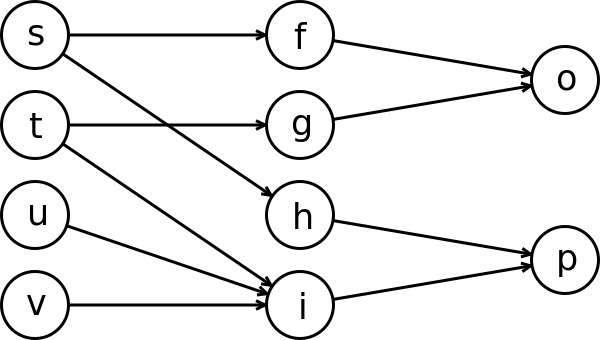
\includegraphics[scale=0.25]{intro_example}
\caption{
    Illustrative example of a dataset to which truth discovery can be applied
    with data sources $\{s, t, u, v\}$, facts $\{f, g, h, i\}$ and objects
    $\{o, p\}$
    \todo{Tikzify, natural language version, present claims as $c: o = v$,
    bipartite graph with objects just indicated}
}
\label{td_new_fig_intro_example}
\end{figure}

\section{Preliminaries}

In this section we give the basic definitions which form our formal framework.
Intuitively, a truth discovery problem consists of a number of \emph{sources}
and a number of \emph{objects} of interest. Each source provides a number of
\emph{claims}, where a claim is comprised of an object and a \emph{value}.
Different sources may give conflicting claims by providing different values for
the same object. For simplicity, we only consider categorical values in this
work. Note that while this restriction is made in some approaches in the
literature \todo{citations}, in general truth discovery methods also handle
continuous values \todo{citations}.

To formalise this, let $\S$, $\O$ and $\V$ be infinite, disjoint sets,
representing the possible sources, objects and values. The input to the truth
discovery problem is a \emph{network}, defined as follows.

\begin{definition}
    A \emph{truth discovery network} is a tuple $(S, O, D, N)$, where
    \begin{itemize}
        \item $S \subseteq \S$ is a finite set of \emph{sources}.
        \item $O \subseteq \O$ is a finite set of \emph{objects}.
        \item $D = \{D_o\}_{o \in O}$ are the \emph{domains} of the objects,
              where each $D_o \subseteq \V$ is a finite set of values. We write
              $V = \bigcup_{o \in O}{D_o}$.
        \item $N \subseteq S \times O \times V$ is a set of \emph{reports}.
    \end{itemize}
    such that
    \begin{enumerate}
        \item\label{td_new_item_val_in_domain}
            For each $(s, o, v) \in N$, we have $v \in D_o$.
        \item\label{td_new_item_sources_self_consistent}
            If $(s, o, v) \in N$ and $(s, o, v') \in N$, then $v = v'$.
    \end{enumerate}
\end{definition}

Note that while $\S$, $\O$ and $\V$ are infinite, each network is finite. The
set $N$ is the core data associated with the network: we interpret $(s, o, v)
\in N$ as source $s$ claiming that $v$ is the true value for object $o$.
Constraint \cref{td_new_item_val_in_domain} says that all claimed values are in
the domain of the relevant object. Constraint
\cref{td_new_item_sources_self_consistent} is is a basic consistency notion: a
source cannot provide distinct values for a single object. That is, a source
provides \emph{at most one value} per object. Thus, while sources may be in
conflict with \emph{other sources}, they are not in conflict with themselves.
This is a simplifying assumption, and is not universal in the literature; e.g.
\todo{find references}. Nevertheless, we argue the truth discovery problem is
still rich enough when conflicts only arise between distinct sources.

A \emph{claim} is a pair $c = (o, v)$, where $o \in O$ and $v \in D_o$. We
write $C$ for the set of claims in a network. With slight abuse of notation, we
write $(s, c)$ for the report $(s, o, v)$. Then $N$ can also be viewed as a
subset of $S \times C$, i.e. a relation between sources and claims. In fact, we
will take this claim-centric view in the remainder of the paper, with objects
and values only playing a role insofar as they tell us which claims are in
conflict with one another.

\begin{example}
    The network illustrated in \cref{td_new_fig_intro_example} is given by $S =
    \{s, t, u, v\}$, $O = \{o_1, o_2\}$, \todo{write when example is polished}
    % \[
    %     N = \{
    %         (s, c), (s, e),
    %         (t, d), (t, f),
    %         (u, f),
    %         (v, f)
    %     \}.
    % \]
\end{example}

We will abuse notation by denoting a network by its data component $N$, with
$S, O$ and $D$ left implicit.
%
The following notation is convenient to
extract the sources associated with a claim and vice versa: for $c \in C$ and
$s \in S$, write
\begin{align*}
    \src_N(c) &= \{s \in S \mid (s, c) \in N\},\\
    \claims_N(c) &= \{c \in C \mid (s, c) \in N\}.
\end{align*}

With the input defined, we come to the output of the truth discovery problem.
The primary goal is to produce as assessment of the trustworthiness of the
sources, and the \emph{true values} for the objects. Approaches differ
regarding values: some truth discovery methods output only a single value for
each object~\cite{li2016,ding_finding_2016,yang_continuous_2018}, whereas
others give as assessment of the believability (or confidence, probability
etc\ldots) of \emph{each claim} $(o,
v)$~\cite{yin2008,pasternack2010,galland2010,zhi2015,zhang_robust_2016,zhang2018}.
We opt for the latter, more general, approach.

On the specific form of these assessments, we face a tension between the social
choice and truth discovery perspectives. In social choice theory, one generally
looks at \emph{rankings}: e.g. the ranking of candidates in an election result
according to a voting rule. Consequently, axioms are generally \emph{ordinal
properties}, which constrain how candidates (for example) compare
\emph{relative to each other}. In contrast, truth discovery methods universally
use \emph{numeric values}. This is more convenient for defining and using truth
discovery methods in practise, and induces a ranking by simply comparing the
numeric scores. However, numeric scores are often not comparable between
different methods (for example, some methods output probabilities, whereas
others are interpreted as weights which may take negative values) and in
general may not carry any semantic meaning at all. This means that meaningful
axioms for truth discovery should not refer to specific numeric scores, but
only the ranking they introduce. \todo{caveat: scores give confidence
estimations.}

We will ultimately take a hybrid approach: our methods and example will be
defined in terms of numeric scores, but the axioms will only refer to ordinal
properties. This approach is summarised succinctly by \textcite{altman2008},
who write of ranking systems: ``We feel that the numeric approach is more
suitable for defining and executing ranking systems, while the global ordinal
approach is more suitable for axiomatic classification."

An \emph{operator} maps each network to score and claim scores.

\begin{definition}
    A \emph{truth discovery operator} $T$ maps each network $N$ to a function
    $T_N: S \cup C \to \R$.
\end{definition}

Intuitively, the higher the score $T_N(s)$ for a source $s \in S$, the
\emph{more trustworthy} $s$ is, according to $T$ on the basis of $N$.
Similarly, the higher $T_N(c)$ for a claim $c \in C$, the \emph{more
believable} $c$ is deemed to be. We define the source and claim rankings
associated with $T$ and $N$ by
\begin{align*}
    s \sle_N^T s' &\iff T_N(s) \le T_N(s'), \\
    c \cle_N^T c' &\iff T_N(c) \le T_N(c').
\end{align*}
Then $s \sle_N^T s'$ if $s'$ is at least as trustworthy as $s$, and similar for
$\cle_N^T$. Note that $\sle_N^T$ and $\cle_N^T$ are total preorders. We denote
the strict parts by $\slt_N^T$ and $\clt_N^T$ respectively, and the symmetric
parts by $\seq_N^T$ and $\ceq_N^T$. We omit the sub- and super-scripts when
$N$ and $T$ are clear from context.

\section{Example Operators}

Our framework is general enough to capture several methods from the truth
discovery literature. In this section we provide two concrete examples: a
baseline voting method and its generalisation to weighted voting, and
Sums~\cite{pasternack2010}. \todo{Can we define some more?} We go on to define
the class of \emph{recursive operators} -- of which Sums is an instance --
which contains many more examples from the literature.

\subsection{Voting}

It is common in the literature to evaluate truth discovery methods against a
non-trust-aware method, such as a simple voting procedure.\footnotemark{} Here
we consider each source to ``vote" for their claims, and claims are ranked
according to the number of votes received, i.e. by $|\src_N(c)|$. While this
ignores the trust aspect of truth discovery entirely, this method will be
useful for us as an axiomatic baseline. For example, axioms which aim to
address the trust aspect should not hold for voting, and an axiom referring to
the ranking of claims may be too strong if it does hold for voting.

\footnotetext{
    This is often called \emph{majority voting} in the truth discovery
    literature (e.g.~\cite{li_survey_2016,xiao_22,li2016}), but using the
    terminology of social choice theory it is better described as
    \emph{plurality voting}.
}

\begin{definition}
    $\voting$ is the operator defined by
    \begin{align*}
        \voting_N(s) &= 1,\\
        \voting_N(c) &= |\src_N(c)|.
    \end{align*}
\end{definition}

Applying $\voting{}$ to the network in \cref{td_new_fig_intro_example}, we have
that all sources rank equally ($s \seq t \seq u \seq v$) and $c \ceq d \ceq e
\clt f$.

The problem with $\voting{}$ is that all reports are equally weighted. If we
have a mechanism by which sources can be weighted by trustworthiness, the idea
behind voting may still have some merit. We define \emph{weighted voting} as
follows.

\begin{definition}
    A \emph{weighting} $w$ maps each network $N$ to a function $w_N: S \to \R$.
    The associated \emph{weighted voting} operator $\wvoting{w}$ is defined by
    \begin{align*}
        \wvoting{w}_N(s) &= w_N(s), \\
        \wvoting{w}_N(c) &= \sum_{s \in \src_N(c)}{w_N(s)}.
    \end{align*}
\end{definition}

Note that a weighting is essentially just half of a truth discovery operator,
where we only output scores for sources. This is completed to an operator
$\wvoting{w}$ by letting the score for a claim be the sum of the weights of its
sources. ``Untrustworthy" sources are those with $w_N(s) < 0$, since reports
from such sources \emph{decrease} the credibility of a claim.

\begin{example}
    \label{td_new_ex_weighted_voting}
    Set
    \[
        w_N(s) = \frac{1}{|\claims_N(s)|}{
            \sum_{c \in \claims_N(s)}{
                |\src_N(c)|
            }
        }.
    \]
    Then the weight assigned to a source $s$ is the average number of sources
    agreeing with the claims of $s$. Taking $N$ from
    \cref{td_new_fig_intro_example}, we have $w_N(s) = 1$, $w_N(t) = 2$,
    $w_N(u) = 3$, $w_N(v) = 3$.  Consequently,
    \begin{align*}
        \wvoting{w}_N(c) &= w_N(s) = 1,\\
        \wvoting{w}_N(d) &= w_N(t) = 2,\\
        \wvoting{w}_N(e) &= w_N(s) = 1,\\
        \wvoting{w}_N(f) &= w_N(t) + w_N(u) + w_N(v) = 8,
    \end{align*}
    yielding the rankings $s \slt t \slt u \seq v$ and $c \ceq e \clt d \clt
    f$. Note that claim $d$ fares better here than with $\voting$ due to its
    association with source $t$, who is more trustworthy than $s$.
\end{example}

\subsection{Sums}

Sums~\cite{pasternack2010} is a simple and well-known operator adapted from
the \emph{Hubs and Authorities}~\cite{kleinberg1999} algorithm for ranking web
pages. The algorithm operates iteratively and recursively, assigning each
source and claim a sequences of scores, with the final score taken as the
limit of the sequence.

The premise is to extend the linear sum of weighted voting to both claim and
source scores: we iteratively update the score of each source as the sum of the
scores of its claims, and update the score of each claim as the sum of the
scores of its sources. To prevent scores from growing without bound, they are
normalised at each iteration by dividing by the maximum score (for sources and
facts separately).

\begin{definition}
    $\sums$ is the operator defined by $\sums_N(z) = \lim_{n \to
    \infty}{T_N^n(z)}$, for $z \in S \cup C$, where $T_N^0 \equiv
    \frac{1}{2}$, and
    \begin{align*}
        T_N^{n+1}(s) &=
            \frac{1}{Z_S}
            \sum_{c \in \claims_N(s)}{
                T_N^n(c)
            }
        \\
        T_N^{n+1}(c) &=
            \frac{1}{Z_C}
            \sum_{s \in \src_N(c)}{
                T_N^{n+1}(s)
            }.
    \end{align*}
    where $
        Z_S = \max_{t \in S}{
            \left|
                \sum_{c \in \claims_N(t)}{
                    T_N^n(c)
                }
            \right|
        }
    $ and $
        Z_C = \max_{d \in C}{
            \left|
                \sum_{s \in \src_N(d)}{
                    T_N^{n+1}(s)
                }
            \right|
        }
    $ are normalisation factors.
\end{definition}

Returning again to the network $N$ from \cref{td_new_fig_intro_example}, one
can show $\sums_N(s) = 0$, $\sums_N(t) = 1$ and $\sums_N(u) = \sums_N(v) =
\sqrt{2} / 2 \approx 0.7071$, giving a source ranking $s \slt u \seq v \slt t$.
For claims, we have $\sums_N(c) = \sums_N(e) = 0$, $\sums_N(d) = \sqrt{2} - 1
\approx 0.4142$ and $T_N(f) = 1$, giving a claim ranking $c \ceq e \clt d \clt
e$. Note that the claim ranking is identical to that of
\cref{td_new_ex_weighted_voting}. For sources, we see that $t$ moves strictly
upwards in the ranking compared to \cref{td_new_ex_weighted_voting}.
Intuitively, this is because source $t$ claims a superset of the claims of $u$
and $v$, so receives more weight from its claims at each iteration.

\subsection{Recursive Operators}

%-----------------------------------------------------------------------------%

% Framework: - Key concept is that of a *source* making *claims* about an
% *object*.  - An operator ranks sources by trustworthiness, and claims by
% their believability.  - We abstract away the possible values for an object -
% Thus, the value associated with a claim (v, o) is not important: it is only
% important when two claims are in *conflict* - Accordingly, we consider claims
% as primitive objects and assume there is a conflict (equivalence) relation.
% Conceptually, each equivalence class is an object, and the claims within are
% possible values.

%     - Formally:
%         * \S, \C are countably infinite sets of source and claim labels
%         * A network is a tuple (S, C, R, N)
%             - S ⊆ \S is a finite set of sources
%             - C ⊆ \C is a (finite?) set of claims
%             - R is an equivalence relation on C
%             - N ⊆ S x C: (s, c) ∈ N iff s claims c
%           subject to the constraint
%             (s, c), (s, d) ∈ N ⇒ ¬(c R d),
%           i.e. no source provides conflicting reports

%     - Comments:
%         * Values are important in other TD works. E.g. to average reported
%           values in \R^d
%         * (C, R) is a special case of an argumentation framework with clusters
%           of mutually attacking arguments

%     - Operator:
%         * An operator T maps each network (S, C, R, N) to a function
%           T_N: S ∪ C -> \R
%         * We use numerical outputs for convenience when defining operators,
%           although we are generally only interested in *ordinal* properties of
%           the rankings on S, C introduced by T_N

% Operators:
%     - Weighted Voting
%     - Sums
%     - Others?
%     - Recursive operators (T_0, U)
%     - If C finite, a recursive operator converging pointwise converges
%       uniformly. Thus, if U is continuous we have the fixed-point property T* =
%       U(T*)
%     - Show that U_Sums is continuous
%     - [In fact, maybe defer this stuff to axiom satisfaction section?]

% Axioms:
%     - Key principle: the more trustworthy a claim's sources, the more
%       believable the claim. Conversely, the more believable a source's claims,
%       the more trustworthy the source.

%     - Express this via *Coherence*.

%     - Notation: if ≤ is a tpo on a set X, let ≤_pw be the "pairwise" preorder
%       on 2^X defined by
%         A ≤_pw B iff ∃f : A -> B bijective st for all x ∈ A, x ≤ f(x)

%     - Given a network N and operator T, let ≤_coh be the preorder on C defined
%       by
%         s ≤_coh s' iff claims_N(s) ≤NT_pw claims_N(s')
%       Similarly, let ≤_coh be the preorder on C defined by
%         c ≤_coh c' iff src_N(c) ≤NT_pw src_N(c')

%     - Coherence:
%         ≤NT extends ≤_coh, and likewise for strict parts

%     - Give example on intro network
%     - Coherence consequences:
%         * If claims_N(s) = claims_N(s') then s ~= s': weak form of symmetry
%         * Marginal effects of a single claim: if claims_N(s) = Y ∪ {c} and
%           claims_N(s') = Y ∪ {c'}, for some Y ⊆ C, then s ≤NT s' iff c ≤NT c'
%         * Strict part: we have s <_coh s' iff ∃f st c <NT f(c) for some c
%     - Limitation: we can only apply coherence to sources/claims with the same
%       number of claims/sources. We extend this later

%     - Symmetry: straightforward

%     - Independence:
%         - Naive indep (aka strong independence): claim it is bad on the basis
%           of example network with symmetry and informal reasoning (will
%           formalise later?)
%         - PCI: restrict to connected components
%         - Marginal independence: suppose
%             src(c) = X ∪ Y; src(d) = X ∪ Z
%             src(c') = X' ∪ Y; src(d) = X' ∪ Z
%           where X disjoint from Y, Z, sim. for X'. Then c ≤ d iff c' ≤ d'

%           (Q: does the version of MI for sources make sense?)

%         - Come up with some example

%     - Monotonicity properties:
%         - Naive positive responsiveness: new claim for c from s improves c
%           relative to d which c already dominated
%         - Naive monotonicity: claims(c) ⊆ claims(c') ⇒ c ≤ c'
%         - Both are naive because additional sources might be malicious: this
%           could *detract* from the credibility of c'
%         - However, there is a special case where such axioms are appropriate:
%           if N contains only a single object, each source can make at most one
%           claim. In the absence of any other structure we claim a plurality
%           approach is appropriate.
%         - (Introduce single-object pos-resp. With symmetry this implies
%           single-object monotonicity).
%         - Returning to the general case: how do we determine whether a source
%           (or coalition of sources) is malicious? We can use the ideas in MI: X
%           ⊆ S is untrusted if there is an instance of X having a negative
%           marginal effect
%         - Introduce relations R_∃, R_∀ on 2^S:
%             Y R_∃ Z iff ∃ c, d, X st src(c) = X ∪ Y, src(d) = X ∪ Z and c ≤NT d
%             Y R_∀ Z iff ∀ c, d, X st src(c) = X ∪ Y, src(d) = X ∪ Z,
%                         we have c ≤NT d
%         - Claim (to check): MI iff R_∃ ⊆ R_∀
%         - We can extract various notions of trustworthiness of coalitions:
%             * X trustworthy if ∅ R_∀ X (there is no evidence that X strictly
%               worsens some claim)
%             * Less credulous option: X trustworthy if ∅ R_∀ X and ∅ R_∃ X:
%               additionally require some positive evidence as well as just the
%               lack of negative evidence
%             * X untrustworthy if X R_∃ ∅
%             * An individual source s could be said to be untrustworthy if
%                 i) {s} is untrustworthy
%                 ii) s is contained in some ⊆-minimal untrustworthy set
%             * Sim., s could be said to be trustworthy if
%                 i) {s} is trustworthy
%                 ii) s is not contained in any ⊆-minimal untrustworthy set
%             * These probably leave the option of s being neither trusted nor
%               untrusted
%         - These notions allow more nuanced monotonicity properties:
%             * Trust-based mon: if claims(c') = claims(c) ∪ Y for a trustworthy
%               coalition Y, then c ≤ c'
%             * Trust-based positive responsiveness: if s trustworthy, additional
%               claim from s boosts believability

%     - Using the conflict relation:
%         - Anti-coherence: the more trusted a claim's detractors, the less
%           believable it should be.

%         - We have an interesting tension between Coherence, Anti-coherence and
%           Single-Object PR and a symmetry-breaking property

%         - Impossibility result

% Axiom satisfaction (and characterisations?):
%     - Uniform-weighted-voting char. by Naive indep, Symmetry, Naive PR
%     - Leads to another impossibility result with Coherence
%     - Sums: analyse by looking at fixed point property?

% Modifying Sums:
%     - Failure of PCI is not good
%     - Show that Sums converges *ordinally*
%     - Do this by noting that omitting the normalisation step does not affect
%       the rankings, and giving proof as before
